\documentclass{report}

%\usepackage{cite}
\usepackage[pdftex]{graphicx}

%\usepackage[cmex10]{amsmath}
%\interdisplaylinepenalty=2500

%\usepackage{array}
%\usepackage{mdwmath}
%\usepackage{mdwtab}

% *** SUBFIGURE PACKAGES ***
%\usepackage[tight,footnotesize]{subfigure}
% subfigure.sty was written by Steven Douglas Cochran. This package makes it
% easy to put subfigures in your figures. e.g., "Figure 1a and 1b". For IEEE
% work, it is a good idea to load it with the tight package option to reduce
% the amount of white space around the subfigures. subfigure.sty is already
% installed on most LaTeX systems. The latest version and documentation can
% be obtained at:
% http://www.ctan.org/tex-archive/obsolete/macros/latex/contrib/subfigure/
% subfigure.sty has been superceeded by subfig.sty.

%\usepackage[caption=false]{caption}
%\usepackage[font=footnotesize]{subfig}
% subfig.sty, also written by Steven Douglas Cochran, is the modern
% replacement for subfigure.sty. However, subfig.sty requires and
% automatically loads Axel Sommerfeldt's caption.sty which will override
% IEEEtran.cls handling of captions and this will result in nonIEEE style
% figure/table captions. To prevent this problem, be sure and preload
% caption.sty with its "caption=false" package option. This is will preserve
% IEEEtran.cls handing of captions. Version 1.3 (2005/06/28) and later 
% (recommended due to many improvements over 1.2) of subfig.sty supports
% the caption=false option directly:
%\usepackage[caption=false,font=footnotesize]{subfig}
%
% The latest version and documentation can be obtained at:
% http://www.ctan.org/tex-archive/macros/latex/contrib/subfig/
% The latest version and documentation of caption.sty can be obtained at:
% http://www.ctan.org/tex-archive/macros/latex/contrib/caption/

\usepackage{url}

\begin{document}

\title{High speed robotic convoying over rough terrain}
\author{Aaron Fineman\\aaron@wpi.edu}
\maketitle

\begin{abstract}
The goal of this project is to apply various high level control algorithms, in particular potential field based methods, for use in robotic convoys. With a priori knowledge of the kinetic models of the other robots in the convoy, the following robots will be able to determine the intended path and trajectory of their leader without the use of explicit communication. Kinematic and dynamic models were created for the robots. This allowed the simulation of movement over rough terrain. The high level control algorithms was implemented on several Khepera III platforms. The convoy used the robot model to traverse over simulated rough terrain.
\end{abstract}



\tableofcontents

\chapter{Introduction}
This project was inspired by searching for ways to control full-scale convoys. This application is commonly seen in military convoy driving, where a line of vehicles must follow each other while maintaining a safe and constant distance. For smaller vehicles, the advantage is the ability to gauge the path ahead, and avoid obstacles that the preceding vehicle failed to detect. In larger convoys, if the leader malfunctions, the convoy may continue unimpeded, rather than become trapped waiting for the leader to continue. However, there are plenty other applications including, but not limited to, transportation inside a factory.


\chapter{Related Work}
\section{Convoying}
Robotic convoying is a significant research problem in mobile robotics. This problem has been addressed from different points of view, e.g., artificial vision, control theory, artificial intelligence, etc. \cite{article:convoy_comm}. Most existing mobile robot systems still involve a single robot working alone, while there are a wide range of potential applications for robots acting in concert \cite{article:convoy_comm}.

The authors of \cite{article:guidance_control} discuss how a following robot imitates its lead robot, where each of the following robots track the angular and linear velocity of its lead robot. They also presented how to convoy with constant distance between robots while analyzing the case as Velocity Pursuit, Deviated Pursuit, and Proportional Navigation.

\section{Potential Fields}
The study of groups of multiple autonomous mobile robots has been of great interest \cite{article:motion_planning_apf}. In high-speed convoying, fast and efficient coordinated maneuvers are a must, as well as quickly processing data to make a decision. Biologists have observed remarkable group-level characteristics in animal aggregations such as swarms, flocks, school and herds \cite{article:motion_planning_apf}. Some of these characteristic are the ability to make very fast and efficient coordinated maneuvers, quickly process data and to cooperatively make decisions. Thus, there is a significant interest within the robotic community, to better understand the biological imperative and exploit it by incorporating similar principles in artificial robot collectives.  

Researchers typically refer to the use of potential field as a means for assisting a robot to move from one initial configuration to a desired final configuration without colliding with any obstacles. Potential fields consist of force vectors, caused by the obstacles or target positions, which may be linear or tangential and they may have characteristics of repulsive, attractive or random, depending on the state of the agent with respect to its environment \cite{article:apf}. It was originally developed as an on-line collision avoidance approach, applicable when the robot does not have a prior model of the obstacles, but rather senses them during motion execution \cite{article:real_time_avoidance_manip}. The most common potential field function is defined as:

$$F(q)=-\nabla(U_a(q)+U_r(q))$$

It is defined over free space as the sum of an $U_a$ attractive potential pulling the robot toward the goal configuration and a $U_r$ repulsive potential pushing the robot away from the obstacles \cite{article:potential_fields_convoy}. This model attempts to find a collision-free, feasible, path in the neighborhood of the initial estimate. The goal is to define a path for the robot to follow, starting from the initial position moving towards the end/goal position calculated by the negative gradient of the entire field. If the start and the goal configurations cannot be connected through a sequence of feasible configurations, the initial path is then assumed not to lead to a solution. The potential field method has increased in popularity for the control of mobile robots, due to its mathematical simplicity \cite{article:potential_fields_convoy}.

\section{Car Models}
In order to study the dynamics of a vehicle system, these are typically modeled as a quarter car, a half car, and a full car.

\subsection{Quarter Car}
%% FIXME source [12]
To model a car, the typical approach is to break it down into smaller parts, and then recombine the parts at the end. To begin with, a quarter car model is created, showing only one wheel, constrained to one dimension (vertical displacement,) and the associated suspension \cite{article:convoy_comm,article:motion_planning_apf}. The quarter car model is shown in figure \ref{fig:quarter_car}. The car body is represented by the mass M and is connected to a suspension system consisting of a spring K and a damper B . The suspension is connected to the tire which is modeled as a mass M and a spring K connecting it to the road.

\begin{figure}[t]
	\centering
	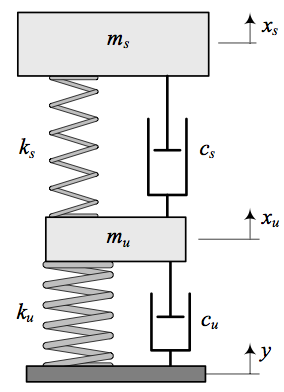
\includegraphics[width=0.25\textwidth]{figures/quarter_car.png}
	\caption{A generalized quarter car model with damped tires \cite{book:jazar}.}
	\label{fig:quarter_car}
\end{figure}

\subsection{Half Car}
The half car model represents a two-dimensional view of the vehicle head-on as shown in figure \ref{fig:half_car}. It is actuated in two dimensions, vertical displacement and rotation about the center of gravity. Horizontal motion (slip) may also be shown on this model. As can be seen from the figure, the half car model is composed of two quarter car models acting on a common strut to realize roll.

\begin{figure}[t]
	\centering
	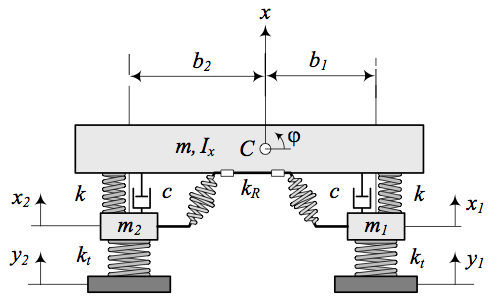
\includegraphics[width=0.7\textwidth]{figures/half_car.png}
	\caption{A generalized half car model with a roll-bar \cite{book:jazar}.}
	\label{fig:half_car}
\end{figure}

\subsection{Full Car}
Full Car. The full car model represents a three-dimensional view of the vehicle as shown in figure \ref{fig:full_car}. The full car model is composed of two half car models, one representing each side (front and back.) From these models one gets a combined roll and pitch. There is then a third (top down) view added to the model that allows for the calculation of yaw, and factors the input velocity into the model.

\begin{figure}[t]
	\centering
	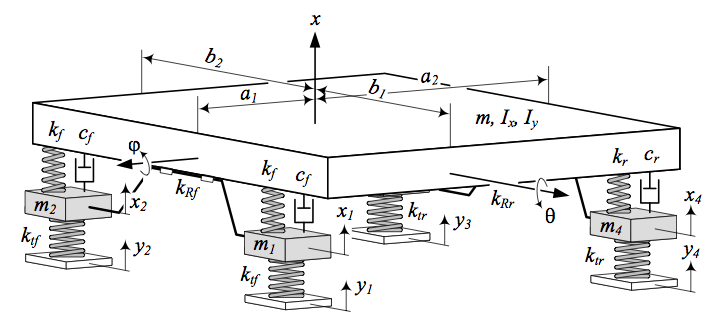
\includegraphics[width=0.9\textwidth]{figures/full_car.png}
	\caption{A generalized full car model with roll-bars \cite{book:jazar}.}
	\label{fig:full_car}
\end{figure}


\chapter{Methodology}
\section{Potential fields}
The goal of this project is to apply various high-level control algorithms, in particular potential field based methods, for use in robotic convoys driving at high speed over rough terrain. As an initial step, the following algorithm to control the convoy was developed and implemented on three Khepera III robots. The trajectory of motion was generated using a potential field algorithm.

Due to hardware limitations, the Khepera robots were only used to simulate the potential field control algorithm. The robot's lack the ability to traverse rough terrain, therefore the high speed convoying and rough terrain navigation was simulated through MATLAB.

The potential field control algorithm was implemented in MATLAB. It is capable of successfully leading n-number of robots from the start position to the goal, assuming that the wheeled mobile robots move in the horizontal plane. The aim was to design a control law for n number of unconnected wheeled autonomous robots to follow a lead robots trajectory generated from the potential field algorithm, while maintaining a constant distance from each other. The control algorithm utilizes the potential field force equation \eqref{eq:potential_fields} to create a matrix of possible configurations for the movement of the robot. The robots' trajectories are defined by the following control equations:
\begin{equation} \label{eq:pot_lead}
	q_n=q+-K*F(q)q
\end{equation}
\begin{equation} \label{eq:pot_follow}
	q_{n(r)}=q_{(r+1)}-o
\end{equation}

Equation \eqref{eq:pot_lead} determines the lead robots next position ($q_n$) based on its current position ($q$) and the potential field force equation \eqref{eq:potential_fields}. The position $q$ and $q_n$ are 2x1 matrices of the form $[x y]^T$. The following robots' new positions ($q_{n(r)}$) are determined by equation \eqref{eq:pot_follow} for a simple leader-follower simulation. The offset from the lead robot ($q_{(r+1)}$) is $o$, a 2x1 matrix of the form $[x y]^T$ representing the straight-line $x$ and $y$ distance between the two robots.

In addition to a simple leader-follower simulation, a second simulation with a smoothing algorithm was implemented in MATLAB. The smoothing control algorithm accomplishes two goals; first, if a following robots leader disappears (i.e. breaks down) the follower becomes the leader and reaches its goal. Second, the following robots are able to follow a smoother trajectory to the goal. A smoother trajectory has less radical turns and directional adjustments required by the robot. The more follower robots, the smoother the final trajectory becomes. This algorithm uses these two equations for the follower robots:
\begin{equation} \label{eq:pot_follow_force}
	F(q) =
	\begin{cases}
		r=1, & -\nabla(U_a(q)+U_r(q) \\
		r>1, & -\nabla(q_{(r+1)}+U_r(q)
	\end{cases}
\end{equation}
\begin{equation} \label{eq:pot_follow_q}
	q_{n(r)}=q_r+-K*F(q)\dot{q}
\end{equation}

Equation \eqref{eq:pot_follow_force} uses the same potential field algorithm as the other simulation except for follower robots, where instead of the attractive field being assigned by the goal position; the attraction is defined by the robot's respective leader's position. For each time step, the robot's leader's position becomes the attractive force \eqref{eq:pot_follow_force} and a new position $q_{n(r)}$ is calculated based on it \eqref{eq:pot_follow_q}. Using this method, the following robots follow smoother trajectories because they react to the information learned by their leader about the terrain. It also solves the issue of a leader robot breaking down; the following robot becomes the new leader and successfully reaches the goal.

The Khepera III's that were used to implement the potential fields simulation use the standard differential drive method. The kinematic equations for this type of robot are:
\begin{eqnarray} \label{eq:diff_drive}
	\dot{x_i} &=& v_i(t)\cos\theta_i\\
	\dot{y_i} &=& v_i(t)\sin\theta_i\\
	\dot{\theta_i} &=& \omega_i(t)
\end{eqnarray}

where $(x_i,y_i)$ are the coordinates of the reference point of i-th robot in the Cartesian frame of reference. $\theta_i$ is its orientation angle with respect to the positive x-axis. $v_i$ and $\omega_i(t)$ are the linear and angular velocities, respectively.

\section{Robot tracking}
To calculate the current location of the robot in the world based off the current ground elevation and/or disturbances, the dynamics of the system are required. The dynamics of car based systems take on the following characteristic form:
\begin{equation} \label{eq:car_characteristic}
[M]\ddot{x}+[b]\dot{x}+[k]x=F
\end{equation}

where $[M]$ are the mass coefficients, $[b]$ are the damping coefficients, and $[k]$ are the spring coefficients. The full realization of this characteristic equation may be seen in appendix \ref{a:dynamics}.

Knowing the position and changes in the center of mass of the vehicle, equation \eqref{eq:car_characteristic} may also be used to calculate the inverse dynamics of the system. This allows for a following vehicle to be able to calculate the ground input on the leading vehicle based off it's movements.


\section{Results}


\chapter{Conclusion}
This document outlined the development of a full control problem of a convoy of high speed robots over rough terrain. It presented the use of a Potential Fields algorithm to control the convoy, while generating a trajectory reference for the robots to follow. Assuming the availability of a priori kinetic models of the other vehicles in the convoy, the followers were able to determine the intended trajectory of their leader without the use of explicit communication.


\section{Future Work}



\addcontentsline{toc}{chapter}{\numberline{}Acknowledgements}
\chapter*{Acknowledgment}
\begin{itemize}
\item Prof. Nestinger
\item Controls group
\end{itemize}


\addcontentsline{toc}{chapter}{\numberline{}Bibliography}
%\bibliographystyle{IEEEtran}
%\bibliography{IEEEabrv,../bib/paper}

\begin{thebibliography}{1}

\bibitem{IEEEhowto:kopka}
H.~Kopka and P.~W. Daly, \emph{A Guide to \LaTeX}, 3rd~ed.\hskip 1em plus
  0.5em minus 0.4em\relax Harlow, England: Addison-Wesley, 1999.

\end{thebibliography}

\appendix
\chapter{Dynamics}



\end{document}

